\chapter{Analysis} \label{chp:analysis}
In order to develop an architecture that eliminates the limitations listed in section \ref{sec:existingsystem:limitations}, an analysis has been done to extract the requirements for the new software components to be used in the new architecture.
This section will develop an analysis to such a degree that the Design chapter can discuss which protocol(s) to use and how the software components should be structured. This chapter starts by listing the assumptions made throughout the project and then proceeds with an analysis of MCLURS and the streaming idea described in section \ref{sec:streamingidea}.

% In order to develop and implement programs to send and receive streams, the requirements from the use cases must be extracted. Some requirements will be logical consequences or decisions in order to nail down details.

\todo{Uses "pub/sub pattern and "topic" " in Streaming idea}

\section{Assumptions}
During the Analysis, Design and Implementation chapters the following assumptions have been made:
\begin{itemize}
	\item No packets are lost or corrupted during transmission. This assumption should hold in relatively small wired networks where no WIFI is in use. Following this assumption, no retransmission of packets will be implemented, and no checksum will be calculated.
	\item No bandwidth limitation exists on the network. Since most network equipment and Ethernet cables are 1 Gbit/s, and this system concerns streams that consume $\approx$ 48 Mbits/s(6MB/s see section \ref{sec:exisingsystem:hardware}), this 1 Gbit/ limitation is ignored. This means that no network congestion control is implemented. 
	
	\item No security is taken into consideration.
		\begin{itemize}
			\item It is assumed that no data is secret or private.
			\item No device on the network tries to tamper with the data.
		\end{itemize}
\end{itemize}

These assumptions are discussed in chapter \ref{chp:discussion}. 

\section{Terminology} \label{sec:analysis:terminology}
Some terminology most be introduced, in order to help the reader throughout the analysis section. Figure \ref{fig:analysis:terminology} shows how data is produced by a \program{Producer}, made into a stream by a \program{Publisher} and streamed to a multicast group. The stream is then received by a \program{Subscriber} which provides the \program{Consumer} with the data  originating from the \program{Producer.}

\begin{figure}[h!]
	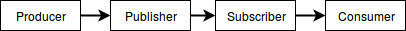
\includegraphics[width=1\textwidth]{figures/analysis-terminilogy-overview.png}
	\caption{Overview of nodes, to help the reader understand the terminology used throughout the following sections. It should be noted that the producer and consumer are just programs producing and consuming streams without being aware of the protocols between the publisher and subscriber.} \label{fig:analysis:terminology}
\end{figure}


\section{Streams} \label{sec:analysis:streams}
A stream is defined as ``A sequence of digitally encoded signals used to represent information in transmission''\citep{data_stream_2018}. A stream does not conceptually have an explicit beginning or end nor does it necessarily have a header explaining the content of the stream.\\
From the uses cases, recordings are finite or potentially infinite streams, in short and long recordings respectively. This implies that streams should be capable of transmitting   continuous media. From \ref{sec:dataanalysis}, a stream can also consist of asynchronous events, implying streams also must be capable of transmitting discrete media. 
A stream can therefore either be continuous or discrete. 
Given use case \ref{sec:usecase:x}, a stream must be capable of comprising  different media such as sound, text or data only by relying on available codecs. 

As mentioned in \ref{sec:streamingidea}, the streams should be transported over multicast groups in order to distribute the streams efficiently, to those network nodes that want them.  This implies that each stream should have its own multicast address, such that a \program{Subscriber} can join that multicast group, and only get that specific stream in order to save bandwidth.

As a logical consequence of using multicast groups, the streams must be transmitted over a  packet-oriented protocol, namely UDP. Even though no packet loss is assumed, the stream must be robust to UDP packets turning up in the wrong order, without losing global knowledge of the stream. TCP is not an option, as this would not take advantage of the multicast groups. TCP is connection-oriented meaning it would require a connection from each \program{Publisher} to each \program{Subscriber}, which would limit the number of \program{Subscribers} per \program{Publisher} since each connection would need full stream bandwidth.

As the stream is just data, there must be metadata available that describes the content of the streams. The streams must be described unambiguously, such that each stream can be differentiated from other streams. The streams must therefore be self-identifying, meaning when a subscriber receives a stream it should already know the properties of the stream such as the media of the stream. The streams must not rely on codecs or formats that put metadata in the beginning of the stream, as this would assume \program{Subscribers} always receive the beginning of a stream, which may not be the case.

Since the streams are to be recorded and replayed, metadata must also be available when the streams are replayed, in order to identify the streams when replayed. Therefore, the streams must be complete and depend on no external knowledge. Analysis of the necessary metadata is conducted in section \ref{sec:analysis:metadata}. When a stream is replayed, it should not necessarily be recorded again. This implies the streams' associated metadata must state whether the stream should not be recorded.

As the system will usually comprise of multiple streams, each stream must have a unique, sensible name used to refer to it. Furthermore it must have an unique identifier that allows streams to refer to each other.
As in \ref{sec:streamingidea}, where a node consumes a stream and produces a new stream, the new stream must explicitly specify its parent stream using the parent's unique identifier. This gives rise to a model of the streams as a forest of graphs, where each graph should always be a directed acyclic graph in order to avoid streams that depend on themselves. An example graph is shown in figure \ref{fig:analysis:graph}

\begin{figure}[h!]
	\centering
	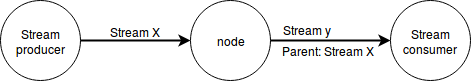
\includegraphics[width=1\textwidth]{figures/stream-graph}
	\caption{Figure showing an example graph of streams. The \program{Publisher} publishes a stream which \program{node} subscribes to. \program{node} then produces an output stream(stream y) which must releate to its parent stream, stream X} \label{fig:analysis:graph}
\end{figure}

Requirements extracted from the analysis are listed in table \ref{tab:requirements}.

\section{Metadata} \label{sec:analysis:metadata}
\subsection{Introduction}

By inspection of the use cases and the streaming analysis in section \ref{sec:analysis:streams}, it has been decided to split metadata into three categories:
\begin{enumerate}
	\item \textit{Essential metadata} covers the metadata that is required to identify and decode the stream.
		An example of this is:
		\begin{itemize}
			\item Sample frequency
			\item Number of channels
			\item Sample size
			\item Encoding(if any)
		\end{itemize}
	\item \textit{Non-essential metadata} is used between the \program{Producer} and \program{Consumer}. This metadata is only relevant to the users.
	\item \textit{Events} describe an event in the stream. An event is defined as something interesting in the stream.
\end{enumerate}

In all three types of metadata, the format must be extensible such that the structure and list of parameters can be modified later on as needed.

It is clear that metadata is essentially hierarchical key-value structures, that can be represented in different formats such as XML, JSON, EBML etc.  From that decision it follows that metadata is:
\begin{itemize}
	\item Extensible -- as new key-value pairs can be added as needed.
	\item Expressive -- since associative arrays, arrays etc. can be expressed.
	\item Convertable -- as both \program{Subscribers} and \program{Publishers} can convert into the format required by the \program{Consumer} and \program{Producer} independently. This is used by Essential metadata in section \ref{sec:analysis:nonessentialmetadata}.
\end{itemize}

When ``metadata'' is used in what follows, it refers to Essential and Non-essential metadata.

\subsection{Essential Metadata} \label{sec:analysis:essentialmetadata}
From the analysis of streams~\ref{sec:analysis:streams}, it is required that the streams are self-identifying to the \program{Subscriber}. This implies that essential metadata describing the properties of the stream must be available unambiguously to the \program{Subscriber}.
From the analysis of streams ~\ref{analysis:stream:requirement:x}, it is required that \program{Subscribers} can join a stream at any arbitrary time. \todo{Followup on this} In order for the \program{Subscriber} to know the properties of the stream, the essential metadata must be retransmitted periodically. As part of the metadata, there must be timestamps that relates to a sample number of the stream. This is required in use case \ref{sec:usecase:drone}, where the recordings are used to do multilateration. In order to not limit the precision of the multilateration, the timestamp must have a precision equal to or lover than the sample period. The maximum sample frequency is 3.08 Mhz, which equals a sample period of $0.33\mu$ seconds\footnote{The sample period might be lower in case hardware with a faster ADC/microcontroller is used}. This metadata is essential in order to identify and decode the stream and will be referred to as ``essential metadata''.


\subsection{Non-essential Metadata} \label {sec:analysis:nonessentialmetadata}
\ac{MCLURS} provides metadata about the recordings which is not essential to identify or decode the stream but is relevant to the user. An example of none-essential metadata is listed in section \ref{sc:existingsystem:setup}. This will be referred to as ``none-essential metadata'', as this metadata is not essential with respect to the streams.
The \program{Publishers} and \program{Subscribers} must be agnostic to the semantics of this metadata, as it is provided by the \program{Producer} and used by the \program{Consumer}. The \program{Subscriber} and \program{Sublisher} must allow for conversion between different formats used by the \program{Producer} and \program{Consumer}, in order to ease implementing \program{Producers} and \program{Consumers}. As with Essential Metadata in section \ref{sec:analysis:essentialmetadata}, the Non-essential metadata must be retransmitted periodically.



%The subscriber and publisher must also be agnostic to the format of the metadata, as the producer and consumer might use XML, JSON, EMBL etc. to represent metadata.

\subsection{Events} \label{sec:analysis:event}
From section \ref{sec:dataanalysis}, it is required that events consists of a timestamp, duration and data. The system must therefore handle events consisting of the following entries:
\begin{itemize}
	\item \textit{Start} States the absolute date and time of when the event appear. 
	\item \textit{Duration} States for how long a time the event is active.
	\item \textit{Data} Associates data to the event. 
\end{itemize}

Given that streams are to be recorded replayable, the events must also be replayable while still relating to a stream and point in time explicitly and unambiguously.


\section{Publishers \& Subscribers} \label{sec:analysis:pubsub}
\subsection{Introduction}
The terminology used to describe types of streams throughout this analysis is used from RFC7656\citep{RFC7656}.

%Nodes publishing streams will be referred to as publishers through the following sections. Nodes receiving streams will be referred to as a subscriber, as they subscribe to streams in order to get the streams. \\
A \program{Subscriber} and \program{Publisher} are depicted in figure~\ref{fig:analysis:pubsub}.

\begin{figure}[h!]
    \centering
    \begin{subfigure}[b]{1\textwidth}
        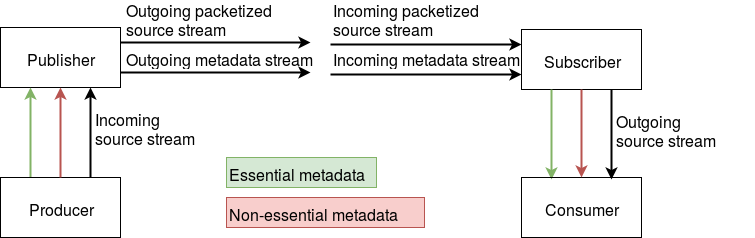
\includegraphics[width=\textwidth]{figures/publisher-subscriber}
    \end{subfigure}
     \caption{The  figure shows a \program{Consumer} providing metadata and a source stream to the \pub, which is sent to a \sub, and provided to the \program{Consumer}}\label{fig:analysis:pubsub}
\end{figure}


A source stream is defined as a stream of digital samples synchronized with a reference clock and coming from a particular media source.

A packetized source stream is defined as a source stream where the stream is split into packets.
The outgoing source stream is identical to the incoming source stream.
Non-essential metadata is as defined in \ref{sec:analysis:metadata}. Incoming Non-essential metadata will be the same key-value pairs as the outgoing non-essential metadata.

The \textit{outgoing metadata stream} is \textit{non-essential} and \textit{essential metadata} combined, as \textit{essential metdata} is generated and used by the \program{Publisher} and \program{Subscriber}. \todo{Correct this.}

\subsection{Analysis} \label{sec:analysis:pubsup:introduction}

From section \ref{sec:streamingidea}, the implementation of the streams follow the Publish-Subscribe pattern. This means two types of interfaces to the streams must exists, namely a \pub{} and \sub{}. The responsibility of the \pub{} is to packetize a source stream, and publish it as a stream. The \subs{} should then be responsible for subscribing to these packeted streams, and provide the source stream to the \con{}.
As streams may contain different media, the \program{Publisher} and \program{Subscriber} must be agnostic to the codec of the stream, and must provide an interface to handle the data as well as metadata to and from the streams.
In order to allow multiple nodes to use a stream, multiple \program{Subscribers} must be able to subscribe to the same multicast group.
If a \program{Publisher} publishes to a multicast group already in use, it must give a warning to the user. In order for this to work, the \program{Publishers} and \program{Subscribers} must implement a presence protocol that detects the presence of other \program{Publishers} and \program{Subscribers} on a specific stream. This must be implemented in a way such that possible conflicts can be detected within X seconds from a \program{Publisher}/\program{Subscriber} is run, where X is specified as a parameter to the nodes of the system.

As there is no designated master in the system, the \program{Publisher} must be designed such that it can find available multicast groups, without relying on too many well-known multicast groups. When a \program{Subscriber} is told to subscribe to a stream using the stream's unique name, the \sub{} must single-handedly be able to find the requested multicast group.
As \program{Publishers} and \program{Subscribers} are unlikely to join multicast groups at the same time, the \program{Publisher} and \program{Subscriber} must be able to cope with nodes asynchronously joining and leaving multicast groups. This implies that \program{Publishers} should periodically resend essential and non-essential metadata to all \program{Subscribers}.
\todo{Fix repeating "resend of metadata periodic"}

From use case \ref{sec:usecase:drone}, the \pubs{} and \subs{} must support being run on the same host. In order for the presence mechanism to know about all publishers and subscribers, each publisher and subscriber most be uniquely named and support having a sensible name set.

Given design requirement X in section \ref{sec:analysis:designrequirements}, the \program{Publishers} and \program{Subscribers} must be opaque such that they encapsulate all of their internal protocols, and hide the streams from the \cons{} and \pros{}. In practice this means that the \program{Producers} and \program{Consumers} must be unaware of the communication between the \program{Subscribers} and \program{Publishers}.


As the \pubs{} and \subs{} should transfer the stream from MCLURS, both \pubs{} and \subs{} must be capable of transferring 6 Mb/s. This means, the \pubs{} and \subs{} must be capable of receiving an input stream of 6Mb/s, and outputting a stream of 6Mb/s.

%Both producer and consumer must be implemented as C-libraries and support bindings to other languages, to ease implementing new consumers and producers for future applications.

%The publishers and subscribers must react to

As essential and non-essential metadata is required, it must be possible to provide essential and non-essential metadata to a \program{Publisher} such that it can send it to the \program{Subscribers}. As \program{Publishers} and \program{Subscribers} can join asynchronously, essential and non-essential metadata must be retransmitted periodically. 
Given that the \program{Subscribers} and \program{Publishers} work on incoming data from either a stream or \program{Producer}, they should only do work if 1) data from a stream is received or 2) the node must do work periodically such as send metadata.

\section{Historian} \label{sec:analysis:historian}

Storing data is essential in all use cases that require post-processing of recordings. Saving recordings to a local disk and later replaying the recordings should be the only responsibilities of a designated node referred to as \program{Historian}.
The \program{Historian} should not be limited to record one stream, but should be capable of saving recordings from multiple streams. 

The historian should be able to save the  three types of recordings, as described in section~\ref{sec:usecase:recordingtypes}:
\begin{itemize}
	\item Long recordings:
		In order for the node to save long recordings, it should be capable of writing to local mounted storage periodically, and not store the entire recording in memory, as this would limit the maximum recording time.

	\item Short recordings:
		With short recordings, the same applies as longtime recordings; however, it should be possible to decide when and for how long a time the recording should run. The historian must provide an interface that allows setting when to do recordings and for how long.
		
	\item Trigger recordings:
		From use case \ref{usecase:trig}, trigger recording is required. The \program{Historian} must be able to replay a recording of arbitrary length at a arbitrary time of recorded data. This implies that the \program{Historian} must support recording while replaying recordings. For this to work, it must be possible to specify which interface the \program{Historian} should replay the recordings to.
\end{itemize}

As the \hist{} should be responsible for recording multiple streams, it should save the streams unambiguously with their associated non-essential and essential metadata, such that the streams can be uniquely identified when replayed.
Given that streams can contain different media, the \hist{} must be agnostic to the content of the stream and to its non-essential metadata.

Given that some streams must not be recorded, the \program{Historian} must support ignoring streams that explicitly state not to be recorded.


\subsection{Replaying}
As introduced in section \ref{sec:streamingidea}, nodes processing streams can either be run when the recordings are happening(online) or when the streams are replayed(offline). In order for this to work, the \program{Historian} must replay streams such that the processing nodes are unaware of the streams are online or offline. This further implies that the content of the streams must be replayed in same order as it was recorded and support real-time replaying meaning x seconds of recording takes x seconds to replay. Furthermore, this implies that metadata recorded must be replayed with the streams. From section~\ref{sec:streamingidea} it is required to be able to replay the same recordings multiple times. This implies that the \program{Historian} must not delete the recordings after the recording has been replayed the first time.
As the \program{Historian} saves streams and metadata with respect to time, the replaying must be started by requesting a replay from a given time and date. It should also be possible to request for how long a period the \program{Historian} should replay streams, so that a replay will not continue forever.
Further more, it should be possible to set a replay-rate, such that replaying can happen faster or slower than realtime. For this to work, the \program{Historian} must have an interface that allows requesting the following options:

\begin{itemize}
	\item Date and time from which the \program{Historian} should replay the streams.
	\item Selecting which streams to be replayed.
	\item The interface to which the streams should be replayed.
	\item Replay rate that allows setting how fast the replaying should happen. 
\end{itemize}

As there is no guarantee that all RPis running \ac{MCLURS} are powered up when the \program{Historian} starts recording, the \program{Historian} must be able to discover streams as they become available using the presence mechanism described in section \ref{sec:analysis:pubsub}.
The \program{Historian} should not rely on specific hardware configuration. See section \ref{sec:analysis:network} for analysis of required network.

Due to limited time, the requirements have been split into \textit{Nice to have} and \textit{Must have} in table \ref{sec:analysis:historian:priotable}.

\begin{table}[]
\centering
\resizebox{\textwidth}{!}{%
\begin{tabular}{|l|}
\hline
\textbf{Nice to have} \\ \hline
The \program{Historian} must support recording multiple streams to local mounted storage.                     \\ \hline
The \program{Historian} must support replaying while recording. \\ \hline
The \program{Historian} must be agnostic with respect to the streams' encoding.
The replayed streams must be unambiguous.
The \program{Historian} must replay streams with all of the streams' associated metadata.
The \program{Historian} must be robust to stream packets arriving out-of-order or never arriving.
The \program{Historian} must replay streams' packets in same order as they are recorded.
The \program{Historian} must ignore streams that explicitly state they should not be recorded.
The \program{Historian} must be able to replay streams and metadata in real-time, as they are recorded.
The \program{Historian} must replay streams such that a processing-node cannot tell whether the stream is replayed or live.
The \program{Historian} must support replaying the same stream multiple times.
\textbf{Must have}    \\ \hline
                      \\ \hline
                      \\ \hline
\end{tabular}%
}
\caption{My caption}
\label{tab:analysis:historian:priotable}
\end{table}

\begin{itemize}
	\item The \program{Historian} must support recording multiple streams to local mounted storage.
	\item The \program{Historian} must support replaying while recording.
	\item The \program{Historian} must be agnostic with respect to the streams' encoding.
	\item The replayed streams must be unambiguous.
	\item The \program{Historian} must replay streams with all of the streams' associated metadata.
	\item The \program{Historian} must be robust to stream packets arriving out-of-order or never arriving.
	\item The \program{Historian} must replay streams' packets in same order as they are recorded.
	\item The \program{Historian} must ignore streams that explicitly state they should not be recorded.
	\item The \program{Historian} must be able to replay streams and metadata in real-time, as they are recorded.
	\item The \program{Historian} must replay streams such that a processing-node cannot tell whether the stream is replayed or live.
	\item The \program{Historian} must support replaying the same stream multiple times.
	
	\item The \program{Historian} must have an interface that allows requesting:
	\begin{itemize}
		\item Date and time from which the \program{Historian} should replay the streams.
		\item Selecting which streams to be replayed.
		\item Select which interface the streams should be replayed. 
		\item Replay rate that allows setting how fast the replaying should happen. 
		\item When the \program{Historian} should start and stop recording.
	\end{itemize}
	\item The \program{Historian} must not rely on specific hardware with specific properties.
	\item The \program{Historian} must be able to discover streams using the presence mechanism.
\end{itemize}

%From the analysis, the following requirements are extracted.
%\section{Energy Calculator} \label{sec:analysis:energy}
%\textbf{Just some notes}
%% Node responsible for calculating energy in signal. 
%From use case \ref{sec:usecase:energizer}, the energy calculation should happen from bulk of samples corresponding to 1 ms. To ease the implementation of the energizer-node and future nodes, it should be possible to set the payload size of the publisher node. If the payload length of the stream corresponds to 1 ms of samples, the energizer node do not have to implement a buffer mechanism. If the length of the packet exceeds the practical limits of the network, the producer must give a warning. From the incoming data to the producer, and the outgoing data from the consumer, there should be no limit of the packet sizes.
%\todo{Subscriber can do buffering}

\section{Network} \label{sec:analysis:network}
%As all streams leaving the nodes are timestamped, there are no restrictions on how the devices should be connected on the network. Packets can go through different number of hobs without causing problems, if the timestamps from the streams are used, and not the order the packets are leaving the \program{Historian} during replay.

%To connect multiple hosts on the network, multiple switches can be connected together. If multiple switches are connected, the bandwidth between switches should be handled with care. Each batbox generates 40 Mbit/s of data, so if a 24 ports switch is used to connect 23 batboxes and one \program{Historian}, the link between the switch and the \program{Historian} must be 1 Gbit. If an 48 ports switch is used, 1.8 Gbits is required between the switch and the \program{Historian}. A switch's non-blocking capacity, meaning the bandwidth it can handle at the same time, not always equals the (number of ports) x (the bandwidth of each port).
As stated in \ref{sec:streamingidea}, multicast is used to distribute streams to \program{Subscribers}. The streams could instead be broadcast, which would cause all devices on the network to receive the streams. This is usually unwanted, as this puts more load on the network than necessary. All network attached devices would have to drop the streams, unless they want them. Unicast is also an option, but this would imply that a \program{Publisher} would have to send N streams if N \program{Subscribers} subscribe to the stream, which would put an unnecessary and redundant load on the \program{Publisher} and the network.

As multicast is utilized to distribute streams, each network switch must support the following features in order to handle multicast traffic properly.

\begin{itemize}
	 \item IGMP snooping, in order to avoid broadcasting multicast traffic.
	 \item MLD, the protocol used by IPv6 to join and leave multicast groups.
\end{itemize}
If IPv6 is used, the switches most support both features, otherwise only IGMP snooping is required. If IGMP snooping is not supported, the multicast traffic will be broadcasted to all network attached devices.
If the system scales out enough, limitations might arise such as running out of multicast groups, switches running out of memory to store which ports have joined certain multicast groups and switches congested due to IGMP/MLD messages. However these limitations should not arise in the relative small scale of hosts used in this system. If the streams are to be sent over the internet, one can not assume no bandwidth limitation and no packet loss.

\section{Loopback Multicast Traffic} \label{sec:analysis:localmulticasttrafic}
As in use case \ref{sec:usecase:drone} where a single RPI is used, the \program{Historian} must run on the same \ac{RPi} as the \ac{MCLURS} software. In order for this to work, the multicast traffic must also work on a loopback interface.  \todo{Verify it works on lo-interface}

\section{Requirements}
From the analysis, the following requirements are extracted.
\subsection{Streams}
\begin{enumerate}
	\item A stream can be either continuous or discrete.
	\item A stream must comprise different datatypes only by relying on available codecs.
    \item Streams must be sent in multicast groups.
    \item Each must must have its own multicast group.
	\item A stream must be packet-oriented, stateless and transported over UDP
	\item A stream must be robust to UDP packets that arrive out of order or never arrive.
	\item A stream must be represented unambiguously
	\item A stream must support referring to its parent stream
\end{enumerate}

\subsection{Essential metadata}
\begin{enumerate}
	\item Essential metadata must unambiguously relate to the streams.
	\item Essential metadata must comprise hierarchical key-value pairs.
	\item Essential metadata must be retransmitted periodically
	\item The Essential metadata must contain a timestamp that relates to the sample number. The precision of the timestamp must be within $0.33\mu$ seconds.
\end{enumerate}

\subsection{Non-essential metadata}
\begin{enumerate}
	\item Non-essential metadata must be hierarchical key-value pairs.
	\item Non-essential metadata must unambiguously relate to the streams.
	\item The \program{Publisher} and \program{Subscriber} must be agnostic with respect to the semantics of the non-essential metadata.
	\item The Non-essential metadata must be retransmitted periodically.
\end{enumerate}

\subsection{Events}
\begin{itemize}
	\item Events must have a start time and date
	\item Events must have a duration.
	\item Events must contain data relating to the event.
\end{itemize}

\subsection{Publisher \& Subscriber}
\begin{enumerate}
		\item The \program{Publishers} and \program{Subscribers} must implement a presence mechanism to know about other \program{Publishers} and \program{Subscribers}. The mechanism should have the following properties:
	\begin{enumerate}
		\item It must take a finite maximum number of seconds for a \program{Publisher} or \program{subscriber} to know who is participating in a specific RTP session. This maximum time must be a parameter of each node.
		\item It must take a finite maximum number of seconds for a \program{Publisher} or \program{Subscriber} to detect whether a multicast group is in use, and if yes, by whom.
		\item Nodes leaving a multicast group sends a ``bye''.
		\item It must be robust to ``bye''-messages not arriving to all nodes.
		\item It must handle nodes joining and leaving at any arbitrary time.
		\item Each \pub{} and \sub{} must by identified by a unique name
 		\item Each \pub{} and \sub{} must have a sensible name provided by the user
	\end{enumerate}
	\item Both \program{Publishers} and \program{Subscribers} must be able to cope with nodes joining asynchronously.
	\item The \pubs and \subs should only do work when 1) data is received and must be processed 2) when periodic work must be done.
\end{enumerate}


\subsubsection*{Publisher}
\begin{enumerate}
	\item The \pubs{} must be able to publish to a topic
	\item The \pub{} must be agnostic to the streams payload.
	\item The \program{Publishers} must be able to find unused multicast groups single-handedly.
	\item The \pub must be transparent from the \pro's perspective.
	\item Essential and non-essential metadata must be sent to \program{Subscribers} periodically.
	\item The \pub{} must be capable of sending a stream of 6Mb/s to a multicast group.
\end{enumerate}

\subsubsection*{Subscriber}
\begin{enumerate}
	\item The \subs{} must be able to subscribe to a topic
	\item The \sub{} must be agnostic to the streams payload.
	\item Multiple \subs{} may receive from the same multicast group.
	\item Given the unique name of a stream, a \program{Subscriber} must be able to resolve the multicast address of the stream.
	\item The \sub{} must be transparent from the \con{} perspective.
	\item The \sub{} must be capable of receiving a stream of 6Mb/s from a multicast group.
\end{enumerate}

\subsubsection*{Historian}
\begin{enumerate}
	\item The \program{Historian} must support recording multiple streams to local mounted storage.
	\item The \program{Historian} must support replaying while recording.
	\item The \program{Historian} must be agnostic with respect to the streams' encoding.
	\item The replayed streams must be unambiguous.
	\item The \program{Historian} must replay streams with all of the streams' associated metadata.
	\item The \program{Historian} must be robust to stream packets arriving out-of-order or never arriving.
	\item The \program{Historian} must replay streams' packets in same order as they are recorded.
	\item The \program{Historian} must ignore streams that explicitly state they should not be recorded.
	\item The \program{Historian} must be able to replay streams and metadata in real-time, as they are recorded.
	\item The \program{Historian} must replay streams such that a processing-node cannot tell whether the stream is replayed or live.
	\item The \program{Historian} must support replaying the same stream multiple times.
	\item The \program{Historian} must have an interface that allows requesting:
	\begin{itemize}
		\item Date and time from which the \program{Historian} should replay the streams.
		\item Selecting which streams to be replayed.
		\item Select which interface the streams should be replayed. 
		\item Replay rate that allows setting how fast the replaying should happen. 
		\item When the \program{Historian} should start and stop recording.
	\end{itemize}
	\item The \program{Historian} must not rely on specific hardware with specific properties.
	\item The \program{Historian} must be able to discover streams using the presence mechanism.
\end{enumerate}


